\subsection{Snorken}\label{section:snorken}
Snorken er et åbenlyst problem når man skal opdage søvn ved hjælp af sensorer, idet at en af de primære sensorer der bruges til at bestemme om en person sover er lyd.
Hvis lyden gentagne gange optager snorken vil sandsynlighedens udregningen for denne sensor falde hver eneste gang snorken bliver optaget, og dette er helt klart et problem som skal arbejdes videre på.

Dette problem kan ses på \cref{fig:snorke-vs-ikkesnorken} hvor vi sammenligner personer som vi ved snorker mod en som ikke snorker.

\begin{figure}
\begin{subfigure}{0.49\textwidth}
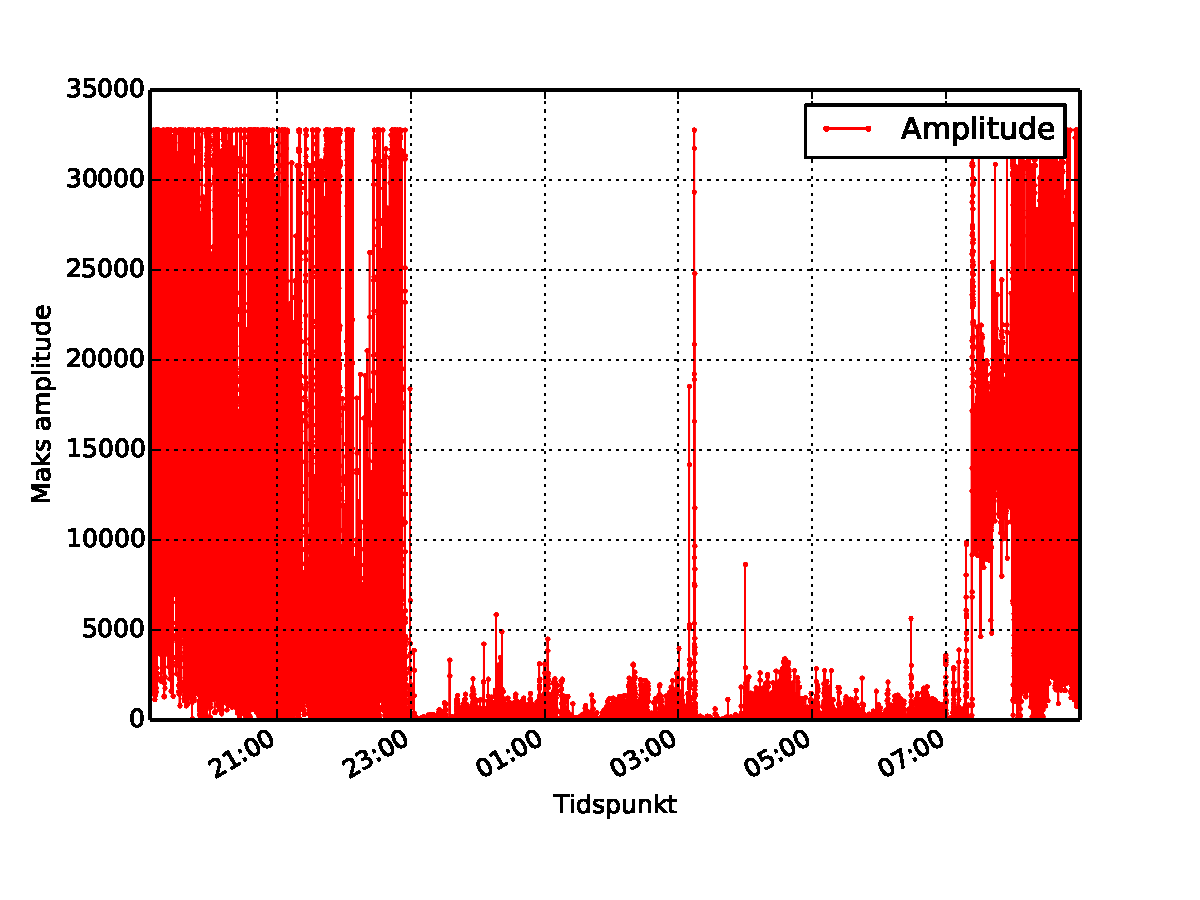
\includegraphics[width=1\textwidth,trim = 1cm 1cm 1cm 1cm,clip]{amplitude-plot-snorken}
\caption{Person der snorker}
\label{fig:person-snorker}
\end{subfigure}
\begin{subfigure}{0.49\textwidth}
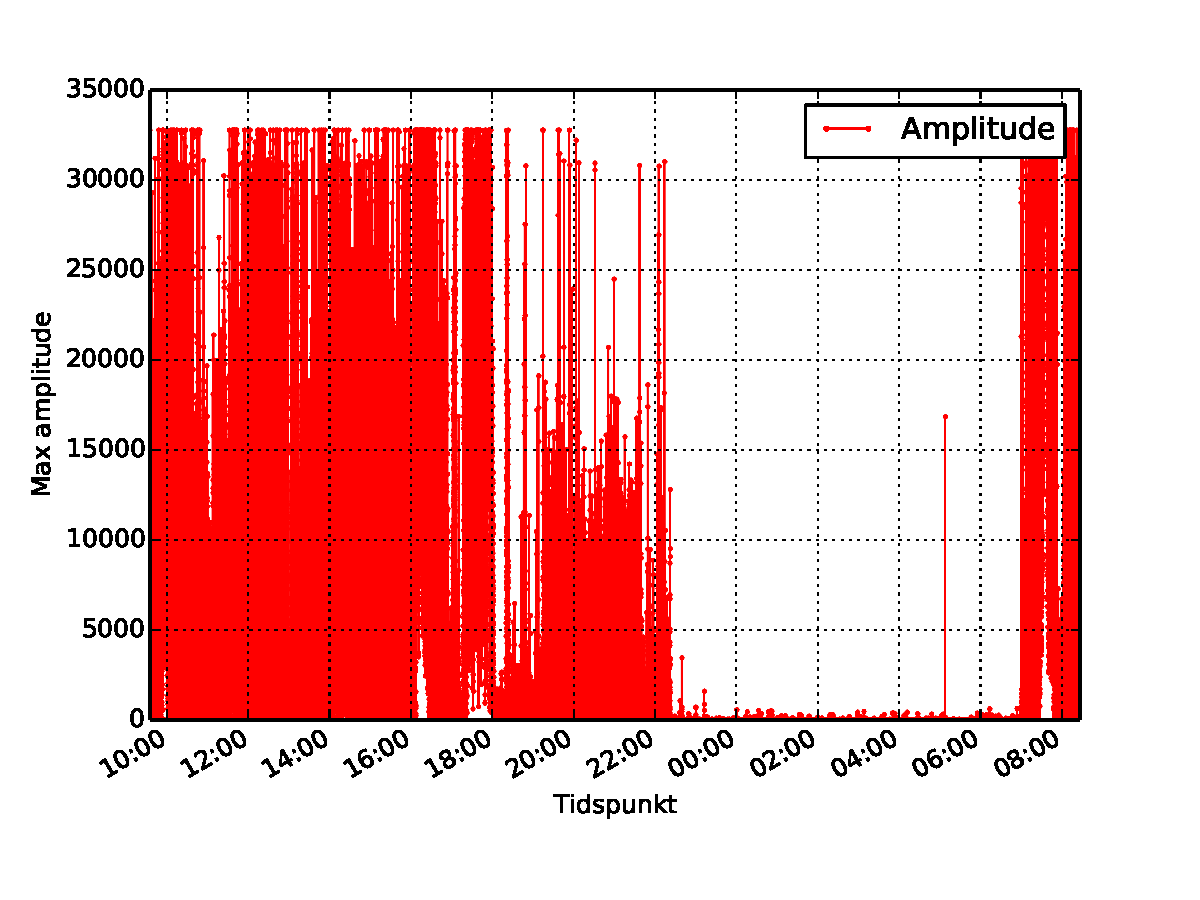
\includegraphics[width=1\textwidth,trim = 1cm 1cm 1cm 1cm,clip]{amplitude-plot}
\caption{Person der ikke snorker}
\label{fig:person-ikke-snorker}
\end{subfigure}
\caption{Person vi ved snorker og person vi ved ikke snorker}
\label{fig:snorke-vs-ikkesnorken}
\end{figure}

Hvis man ser på grafen med snorken, \cref{fig:person-snorker}, kan man klart se at amplituden er mere uregulær i søvn perioden i forhold til grafen i \cref{fig:person-ikke-snorker}. 
En simpel løsning på hvordan man kunne ignorere snorken i sandsynligheds estimeringen ville være at sætte amplitude threshold op på et højere niveau, hvilket baseret på graferne kunne f.eks. være 5000. 
Threshold værdien er den amplitude hvor den betrages som ligegyldig idet at den ikke er høj nok, og kan derfor ses som et 0 når sandsynligheden udregnes. 
Men dette skal være baseret på hvor højt personen snorker og skal derfor være dynamisk, hvilket kan gøre at denne løsning ikke er optimal. Derudover kan man ikke garantere at der ikke findes personer der snorker lige så højt som når de snakker.
Andre metoder på at registrere søvn er derfor undersøgt.

Ud fra artiklerne \citet{Dafna2013}, \citet{Calabrese20111101} og \citet{7051338} dannes der et grundlag for hvordan snorken kan registreres.

\citet{Dafna2013} gør brug af et system til at inddele snorken og andre akustiske hændelser gennem et søvnforløb ved brug af lyd data der blev optaget med en mikrofon ved en polysomnigrafisk undersøgelse. 
De endte med et meget præcist system der kunne adskille snorken og andre akustiske hændelser med ~98\% nøjagtighed.
Denne kunne tilpasses ind i vores system på den måde at hvis snorken kan opdages og filtreres fra har den ikke nogen indflydelse på sandsynligheds beregningen af søvn. 
De bruger lyd data og ikke bare amplituden, så det vil være nødvendigt at undersøge om systemet også kunne fungere ved bare amplituden.

\citet{Calabrese20111101} forslår et system der skal bruges til diagnosticering af søvnapnø ved hjælp af optaget lyd data baseret på analyser af disse, men de implementerede kun en prototype af systemet og havde ikke evalueret systemet ordentligt. 
Idéen her er at man bruger analyser såsom 'Fast Fourier Transform' og 'Power Spectrum' til at finde tidspunkter hvor personen har snorket baseret på optaget lyd. 
Denne metode sår tvivl ved løsningen om blot at indsamle max amplitude, da om nødvendigt skal lydindsamlingen ændres til et sliding window.
Dvs. hvor vi samler det rå lyddata fra mikrofonen, men sletter lyddate efter foretaget analyse, således at privatlivs kriteriet stadig opfyldes.
Dette er en mulighed et modul kan benytte sig af, og bør udforskes med videre arbejde.

\citet{7051338} udvikler et system der kan registrere snorker ud fra lydoptagelser.
Denne metode bruger maskine læring til at udvikle en model til at beskrive hvornår folk de sover.
Den metode de har udviklet bruger en \textit{K}-Nearest Neighbour classifier.
Denne metode kræver ligesom den forrige at vi optager lyd i stedet for bare at se på amplituden.
I modsætning til \citet{Calabrese20111101}, fokuserer \citet{7051338} på det at registrere snorken som dens primære mål, hvilket også kvalificerer denne metode som en oplagt kandidat til videre udforskning.

Hvis man vælger at arbejde videre med en af disse metoder til at detektere snorken, har det også andre anvendelsesmuligheder end at fjerne støj fra vores estimering.
Hvis en af metoderne registrerer at man snorker, kan man sige at det uden tvivl betyder at en person sover, og så kan den procentvurdering der ellers havde været på det tidspunkt bliver overskrevet med 100 \%.
Dette er en meget relevant ting at bruge snorke registrering til, da det vil forbedre nøjagtigheden meget, i stedet for bare at fjerne støj.
